
\newpage
\section{Proof that cluster states need exponentially-large QMDDs}
\label{sec:graph-state-lower-bound}


In this appendix, we formally prove that cluster states have exponential size in \qmdds \autoref{thm:graph-state-qmdd-lower-bound}.
We first fix notation and definitions, after which we prove 
%\autoref{thm:graph-state-qmdd-lower-bound} 
the theorem using two lemmas.

Let $G$ be an undirected graph with vertices $V_G=\{v_1, \dots, v_n\}$ and edge set $E_G \subseteq V_G\times V_G$.
For a subset of vertices $S\subseteq V_G$, the $S$-induced subgraph of $G$ has vertices $S$ and edge set $(S \times S) \cap E$.
Given $G$, its graph state $\ket{G}$ is given in \autoref{eq:graph-state-definition} in \autoref{sec:preliminaries} and can equivalently be expressed as
\[
    \ket{G} = \sum_{\vec x\in \set{0,1}^n} (-1)^{f_G(\vec x) } \ket{\vec x}
\]
where $f_G(\vec{x})$ is the number of edges in the $S$-induced subgraph of $G$.

For a function $f: \{0, 1\}^n \rightarrow \mathbb{C}$ and bit string $\vec a=a_1\cdots a_k\in\{0, 1\}^k$, we denote by $f_{\vec{a}}$ the subfunction of $f$ restricted to $\vec a$:
\begin{align}
f_{\vec a}(x_{k+1},\ldots, x_n) := f(a_1,\ldots, a_k,x_{k+1},\ldots, x_n)
\end{align}
We also say that $f_{\vec a}$ is a subfunction of $f$ of \emph{order} $|\vec a|=k$.
%The string $a$ is called a \emph{partial assignment} to $f$.

We will also need the notions of boundary and strong matching.

\begin{definition}[Boundary]
	For a set $S\subseteq V_G$ of vertices in $G$, the \emph{boundary} of $S$ is the set of vertices in $S$ adjacent to a vertex outside of $S$.
\end{definition}

\begin{definition}[Strong Matching]\label{def:smatch}
	Let $G=(V,E)$ be an undirected graph. A \emph{strong matching} is a
	subset of edges $M \subseteq E$ that do not share any vertices (i.e., it is a matching)
	and no two edges of $M$ are incident to the same edge of $G$, i.e.,
	an edge in $E \setminus M$. Alternatively, a strong matching is a matching $M$ s.t. $G[V(M)] = M$.
	We say that $M$ is an $(S,T)$-strong matching for two sets of vertices $S,T\subset V$ if $M\subseteq S\times T$.
	For a strong matching $M$ and a vertex $v\in V(M)$, we let $M(v)$ denote the unique vertex to which $v$ is matched by $M$.
\end{definition}



%\todo[inline]{
% Write $\chi(x_1, \dots, x_n)$
%be the indicator function for vertices: $\chi(x_1, \dots, x_n) \defn \{v_i \mid x_i=1, i \in [n]\} $.
%Let $f_G\colon \bool^n\to \bool$ be the number of edges in the $S$-induced subgraph of $G$, written $G[S]$, modulo $2$, as in \autoref{eq:induced-subgraph-fn}. 
%\begin{align}
%	\label{eq:induced-subgraph-fn}
%	f_G(x_1,\ldots, x_n)  \defn |G[ \chi(x_1, \dots, x_n)]|\mod 2
%\end{align}
%%Here $E[S]$ is the subgraph induced by the set indicated by the vertices $S \subseteq V$.
%For a graph $G$, the graph state $\ket{\psi_G}$ is defined in terms of $f_G$, namely,
%\begin{align} 
%	\ket{\psi_G} \defn \sum_{\vec x\in \set{0,1}^n} (-1)^{f_G(\vec x) } \ket{\vec x}
%\end{align}
%Then the main result is \autoref{th:graph-state-qmdd-lower-bound}: that the function $f_G$ is difficult for BDDs, and $\ket{\psi_G}$ is difficult for \textsc{QMDD}s.
%}
%
%Given a variable order, a Decision Diagram (DD) is a DAG that uniquely represents a function (see \autoref{sec:preliminaries-dd} for details).
%Each path in a DD represents a (partial) assignment to the first variables
%in the order. 
%We prove \autoref{th:graph-state-qmdd-lower-bound} by counting unique subfunctions (= different DD nodes) induced by
%those partial assignments (for any variable order).
%\autoref{thm:bdd-size-from-subfunctions} and \autoref{thm:qmdd-size-from-subfunctions} show how we translate our count of unique subfunctions to a lower bound on diagram size.

Using these definitions and notation, we prove \autoref{thm:graph-state-qmdd-lower-bound}.

\begin{proof}[Proof of \autoref{thm:graph-state-qmdd-lower-bound}]
%	Consider the set $B_S:=\text{Boundary}(S)$.
%	
Let $G=\text{lattice}(n,n)$ be the undirected graph of the $n\times n$ lattice,
with vertex set $V=\{v_1,\ldots, v_{n^2}\}$.
Let $\sigma=v_1v_2\cdots v_{n^2}$ be a variable order, and let $S=\{v_1,v_2,\ldots, v_{\frac{1}{2}n^2}\}\subset V$ be the first $\half n^2$ vertices in this order.

The proof proceeds broadly as follows.
First, in \autoref{thm:strong-matchings-yield-subfunctions}, we show that any $(S,\overline S)$-strong matching $M$ effects $2^{|M|}$ different subfunctions of $f_G$.
Second, \autoref{thm:large-strong-matching} shows that the lattice contains a large $(S,\overline S)$-strong matching for any choice of $S$.
    Put together, this will prove the lower bound on the number of QMDD nodes as in \autoref{thm:graph-state-qmdd-lower-bound} by the fact that a QMDD for the grid graph state $G$ has a node per unique subfunction of the function $f_G$.
	Figure \ref{fig:strong-matching-in-grid} illustrates this setup for the $5\times 5$ lattice.

\begin{lemma}
	\label{thm:strong-matchings-yield-subfunctions}
	Let $M$ be a non-empty $(S,\overline S)$-strong matching for the vertex set $S$ chosen above.
	If $\sigma=v_1v_2\cdots v_{n^2}$ is a variable order where all vertices in $S$ appear before all vertices in $\overline S$, then $f_G(x_1,\ldots, x_{n^2})$ has $2^{|M|}$ different subfunctions of order $|S|$.
\end{lemma}
\begin{proof}
	Let $S_M:=S\cap V(M)$ and $\overline S_M:=\overline S\cap M$ be the sets of vertices that are involved in the strong matching.
Write $\chi(x_1, \dots, x_n)$ for the indicator function for vertices: $\chi(x_1, \dots, x_n) := \{v_i \mid x_i=1, i \in [n]\} $.
	Choose two different subsets $A,B\subseteq S_M$ and let $\vec{a}=\chi^{-1}(A)$ and $\vec{b}=\chi^{-1}(B)$ be the corresponding length-$|S|$ bit strings.
	%		We will show that $\vec{a}$ and $\vec{b}$ induce different subfunctions.
	%		Let $\vec{a}=a_1,\ldots,a_{\half n^2}$ and $\vec{b}=b_1,\ldots,b_{\half n^2}$ be two different partial assignments which are nonzero only on $S_M$, i.e., for all $v_i\not\in S_M$, $a_i=b_i=0$.
	%		The bit strings correspond to sets $S_{\vec a},S_{\vec b}\subseteq S_M$.
	%		
	These two strings induce the two subfunctions $f_{G,\vec{a}}$ and $f_{G,\vec{b}}$.
	We will show that these subfunctions differ in at least one point.
	
	First, if $f_{G,\vec{a}}(0,\ldots, 0)\ne f_{G,\vec{b}}(0,\ldots, 0)$, then we are done.
	Otherwise, take a vertex $s\in A\oplus B$
    and say w.l.o.g. that $s\in A\setminus B$.
	Let $t=M(s)$ be its partner in the strong matching.
	Then we have, $|E[A\cup \{t\}]| = |E[A]|+1$ but $|E[B\cup \{t\}]|=|E[B]|$.
	Therefore we have 
	%		Then we have 
	\begin{align}
	f_{G,\vec a}(0,\ldots, 0, x_t=0, 0,\ldots, 0) ~~\ne~~ &f_{G,\vec a}(0,\ldots,0,x_t=1,0,\ldots, 0) \\
	f_{G,\vec b}(0,\ldots, 0, x_t=0, 0,\ldots, 0) ~~=~~ & f_{G,\vec b}(0,\ldots, 0,x_t=1,0,\ldots, 0)
	\end{align}
	%		This is because the edge $(s,t)$ is counted in the $\vec a$ subfunction, but not in the $\vec b$ subfunction.
	%		
	We see that each subset of $S_M$ corresponds to a different subfunction of $f_G$. Since there are $2^{|M|}$ subsets of $M$, $f_G$ has at least that many subfunctions.
\end{proof}

We now show that the $n\times n$ lattice contains a large enough strong matching.

\begin{lemma}
	\label{thm:large-strong-matching}
	Let $S=\{v_1,\ldots, v_{\frac{1}{2} n^2}\}$ be a set of $\half n^2$ vertices of the $n\times n$ lattice, as above.
	Then the graph contains a $(S,\overline S)$-strong matching of size at least $\floor{\frac{1}{12}n}$.
\end{lemma}
\begin{proof}
	Consider the boundary $B_S$ of $S$.
	This set contains at least $n/3$ vertices, by Theorem 11 in \cite{lipton1979generalized}.
	Each vertex of the boundary of $S$ has degree at most $4$. 
    It follows that there is a set of $\left\lfloor \frac{1}{4}|B_S|\right\rfloor$ vertices which share no neighbors.
	% todo B_T or \overline S?
	In particular, there is a set of $\left\lfloor \frac{1}{4}|B_S| \right\rfloor\geq \floor{\frac{1}{12}n}$ vertices in $B_S$ which share no neighbors in $\overline S$.
\end{proof}
Put together, every choice of half the vertices in the lattice yields a set with a boundary of at least $n/3$ nodes, which yields a strong matching of at least $\floor{\frac{1}{12}n}$ edges, which shows that $f_G$ has at least $2^{\floor{\frac{1}{12}n}}$ subfunctions of order $\frac{1}{2}n^2$.
\end{proof}

\begin{figure}[h!]
\centering
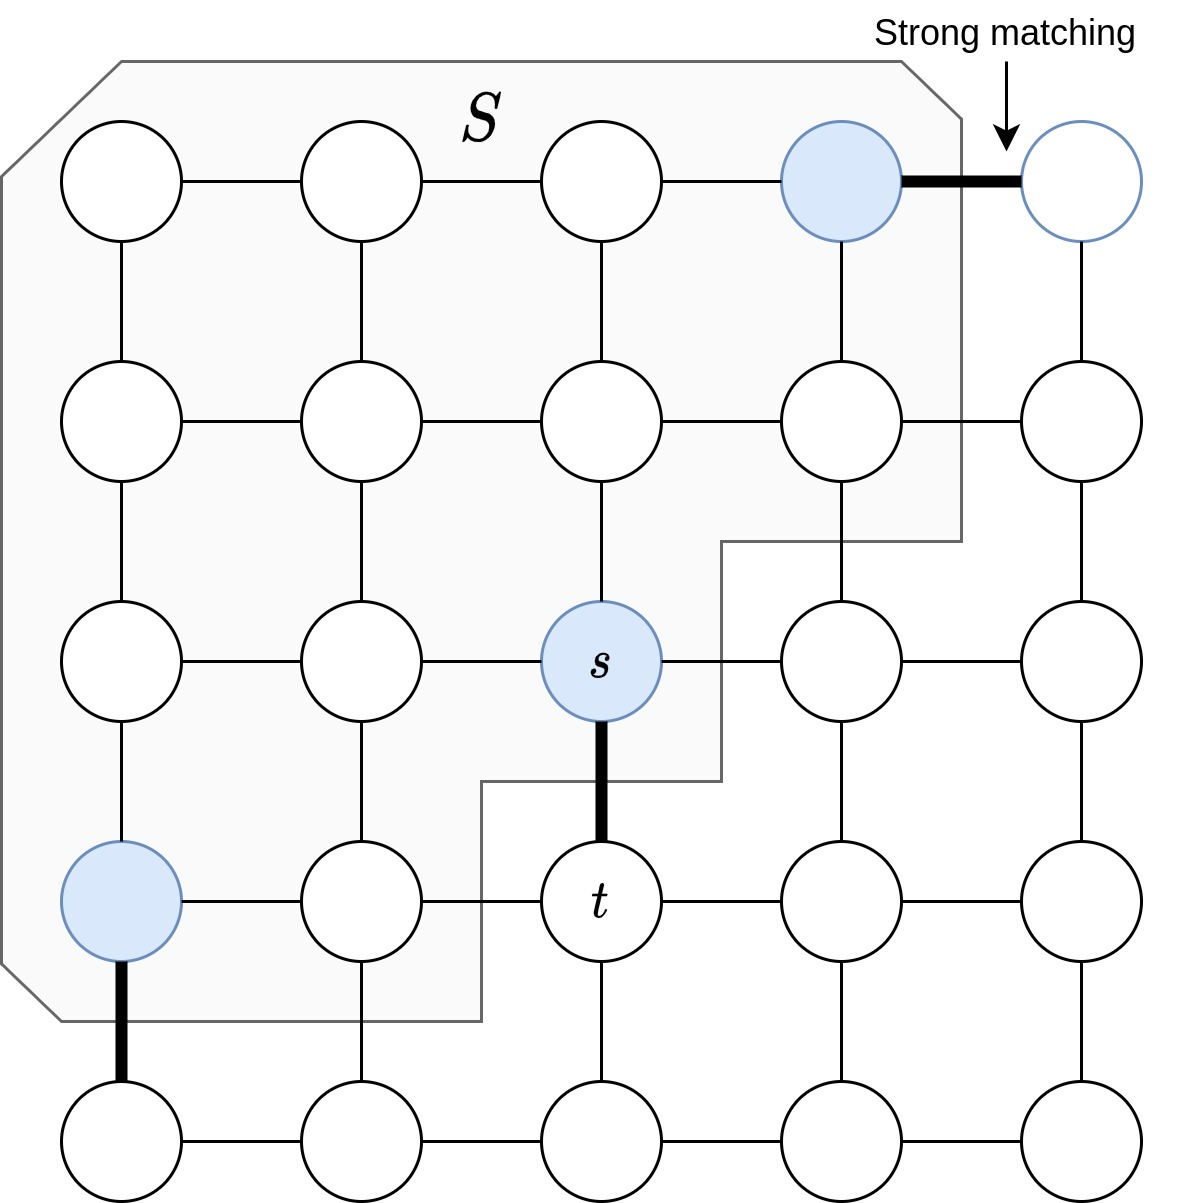
\includegraphics[width=0.45\textwidth]{pics/strong-matching-in-grid.jpg}
\caption{
    The $5\times 5$ grid graph, partitioned in a vertex set $S$ and its complement $\overline{S}$.
    A strong matching between $S$ and $\overline{S}$ is indicated by black edges.
}
\label{fig:strong-matching-in-grid}
\end{figure}


% todo =======================

\subsection{Proof that XOR states need exponentially large QMDDs}

We now show that \qmdds which represent so-called XOR states are exponentially large in the worst case.
On the other hand, in \autoref{sec:graph-states-limdds}, we will show that these states can be represented using only $\mathcal O(n)$ nodes by $\braket{X}$-\limdds, showing that they are exponentially more succinct than \qmdds.
We define XOR states as uniform superpositions over vectors spaces, as follows.

\begin{definition}[XOR-state]
	\label{def:xor-states}
	Let $V\subseteq\{0,1\}^n$ be a vector space, i.e., for every $x,y\in V$ it holds that $x\oplus y\in V$.
	Then the XOR-state $\ket{V}$ is the uniform superposition over the elements of $V$, i.e.,
	\begin{align}
	\ket{V}=\frac{1}{\sqrt{|V|}}\sum_{x\in V}\ket x
	\end{align}
\end{definition}

%The normalization factor $1/\sqrt{|V|}$ is not important to us, because our diagrams do not necessarily normalize a quantum state.
We will use the following result by \v{D}uri\v{s} et al. on binary decision diagrams (\bdds), which are \adds with codomain $\{0, 1\}$.
%The \qmdd lower bound is a corollary to the following result by \v{D}uri\v{s} et al. on binary decision diagrams (\textsf{BDD}s), which are \adds with codomain $\{0, 1\}$.

\begin{theorem}[\v{D}uri\v{s} et al.\cite{vdurivs2004multi}]
	\label{thm:random-vector-space-hard-for-bdd}
	The characteristic function $f_V: \{0, 1\}^n \rightarrow \{0, 1\}$ of a randomly chosen vector space $V$ in $\{0, 1\}^n$, defined as $f_V(x)=1$ if $x\in V$ and  $0$ otherwise, needs a \bdd of size $2^{\Omega(n)}/(2n)$ with high probability.
	%    \todo[inline]{@Lieuwe: should define branching program. Can replace by BDD?}
\end{theorem}

Our result follows by noting that if $f$ is as above, or indeed if $f$ is any function with codomain $\{0, \lambda\}$ for any scalar $\lambda$, then the \qmdd of the state $\ket{f}=\sum_xf(x)\ket{x}$ has the same structure as the \bdd of $f$.
That is to say, in this case, the \bdd and \qmdd are graphs with the same number of nodes.

\begin{corollary}
	\label{thm:random-xor-state-hard-for-qmdd}
	For a random vector space $V\subseteq \{0,1\}^n$, the XOR-state $\ket{V}$ requires \qmdds of size $2^{\Omega(n)}/(2n)$ with high probability.
\end{corollary}
\begin{proof}
	A \bdd encodes a function $f\colon \{0,1\}^n\to\{0,1\}$.
	In this case, the \bdd encodes $f_V$, the characteristic function of $V$.
	A \bdd is a graph which contains one node for each subfunction of $f$.
	
	Similarly, a \qmdd representing a state $\ket{\phi}=\sum_xf(x)\ket{x}$ can be said to represent the function $f\colon\{0,1\}^n\to\mathbb C$, and contains one node for each subfunction of $f$ modulo scalars.
	In this case, it represents the function $1/\sqrt{|V|}f_V\colon \{0,1\}^n\to\{0,1/\sqrt{|V|}\}$.
	However, in the case of $f_V$, two distinct subfunctions are not equal up to a scalar, because the codomain is $\{0,1\}$.
	To this end, let $f_{V,a},f_{V,b}$ be distinct subfunctions of $f_V$ induced by partial assignments $a,b\in\{0,1\}^k$.
	We will show that there is no $\lambda\in\mathbb C^{\ast}$ such that $f_{V,a}=\lambda f_{V,b}$.
	To see this, say that the two subfunctions differ in the point $x\in\{0,1\}^{n-k}$, i.e., $f_{V,a}(x)\ne f_{V,b}(x)$.
	Say without loss of generality that $f_{V,a}(x)=0$ and $f_{V,b}(x)=1$.
	Then, since $\lambda\ne 0$, we have $\lambda=\lambda f_{S,b}(x)\ne f_{V,a}(x)=0$, so $f_{V,a}\ne \lambda f_{B,b}$.
	
	Because distinct subfunctions of $f_V$ are not equal up to a scalar, the \qmdd for $\ket{V}$ contains a node for every subfunction of $f_V$.
	We conclude that, since by \autoref{thm:random-vector-space-hard-for-bdd} with high probability the \bdd representing $f_V$ has exponentially many nodes, so does the \qmdd representing $\ket{V}$.
\end{proof}